\section{Extending Firefox}

When you first download and install Firefox, it can handle basic browser
tasks immediately. You can also add extra capabilities or change the way
Firefox behaves by installing add-ons, small additions that extend
Firefox's power.

Firefox extensions can pimp your browser, but they can also collect and
transmit information about you. Before you install any add-on, keep in
mind to choose add-ons from trusted sources. Otherwise, an add-on might
share information about you without your knowing, keep a record on the
sites you have visited, or even harm your computer.

There are several kinds of add-ons:

\begin{itemize}
\item
  \emph{Extensions} add functionality to Firefox
\item
  \emph{Themes} change the appearance of Firefox.
\item
  \emph{Plugins} help Firefox handle things it normally can't process
  (i.e.~Flash movies, Java applications).
\end{itemize}
For the topics covered in this book we are only going to need
extensions. We will look at some add-ons that are particularly relevant
for dealing with Internet security. The variety of available extensions
is enormous. You can add dictionaries for different languages, track the
weather in other countries, get suggestions for Web sites that are
similar to the one you are currently viewing, and much more. Firefox
keeps a list of current extensions on its site
(\href{https://addons.mozilla.org/firefox}{https://addons.mozilla.org/firefox}),
or you can browse them by category at
\href{https://addons.mozilla.org/firefox/browse}{https://addons.mozilla.org/firefox/browse}.

\textbf{Caution:} We recommend that you never install an add-on for
Firefox unless it is available from the Firefox add-on pages. You should
also never install Firefox unless you get the installation files from a
trusted source. It is important to note that using Firefox on someone
else's computer or in an Internet caf increases your potential
vulnerability. Know that you can take Firefox on a CD or USB-stick
(check our chapter on that issue).

While no tool can protect you completely against all threats to your
online privacy and security, the Firefox extensions described in this
chapter can significantly reduce your exposure to the most common ones,
and increase your chances of remaining anonymous.

\subsection{HTTPS Everywhere}

HTTP is considered unsafe, because communication is transmitted in plain
text. Many sites on the Web offer some support for encryption over
HTTPS, but make it difficult to use. For instance, they may connect you
to HTTP by default, even when HTTPS is available, or they may fill
encrypted pages with links that go back to the unencrypted site. The
HTTPS Everywhere extension fixes these problems by rewriting all
requests to these sites to HTTPS. Although the extension is called
``HTTPS Everywhere'', it only activates HTTPS on a particular list of
sites and can only use HTTPS on sites that have chosen to support it. It
cannot make your connection to a site secure if that site does not offer
HTTPS as an option.

\begin{figure}[htbp]
\centering
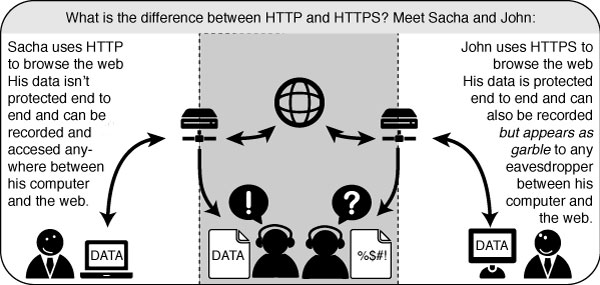
\includegraphics{https_schema.jpg}
\caption{HTTPS Schema}
\end{figure}

Please note that some of those sites still include a lot of content,
such as images or icons, from third party domains that is not available
over HTTPS. As always, if the browser's lock icon is broken or carries
an exclamation mark, you may remain vulnerable to some adversaries that
use active attacks or traffic analysis. However, the effort required to
monitor your browsing should still be usefully increased.

Some Web sites (such as Gmail) provide HTTPS support automatically, but
using HTTPS Everywhere will also protect you from TLS/SSL-stripping
attacks, in which an attacker hides the HTTPS version of the site from
your computer if you initially try to access the HTTP version.

Additional information can be found at:
\href{https://www.eff.org/https-everywhere}{https://www.eff.org/https-everywhere}.

\subsection{Installation}

First, download the HTTPS Everywhere extension from the official Web
site:
\href{https://www.eff.org/https-everywhere}{https://www.eff.org/https-everywhere}

\begin{figure}[htbp]
\centering
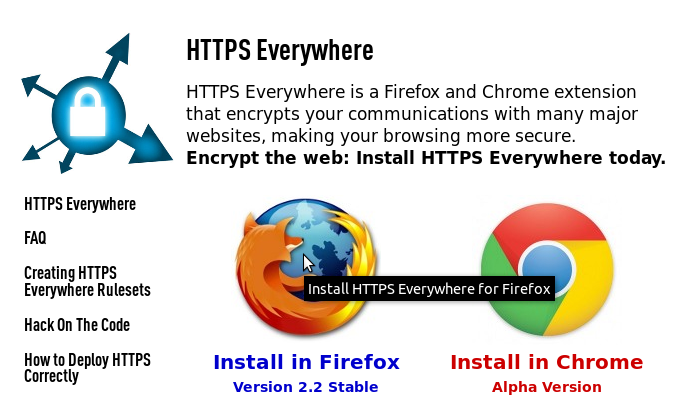
\includegraphics{https_everywhere.png}
\caption{HTTPS Everywhere}
\end{figure}

Select the newest release. In the example below, version 2.2 of HTTPS
Everywhere was used. (A newer version may be available now.)

\begin{figure}[htbp]
\centering
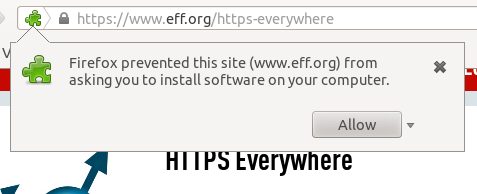
\includegraphics{https_everywhere_2.png}
\caption{HTTPS Everywhere}
\end{figure}

Click on ``Allow''. You will then have to restart Firefox by clicking on
the ``Restart Now'' button. HTTPS Everywhere is now installed.

\subsection{Configuration}

To access the HTTPS Everywhere settings panel in Firefox 4 (Linux),
click on the Tools menu at the top of your screen and then select
Add-ons. (Note that in different versions of Firefox and different
operating systems, the Add-ons Manager may be located in different
places in the interface.)

\begin{figure}[htbp]
\centering
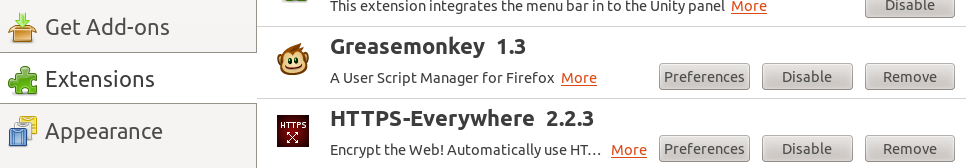
\includegraphics{https_everywhere_3.png}
\caption{HTTPS Everywhere}
\end{figure}

Click on the Preferences button.

\begin{figure}[htbp]
\centering
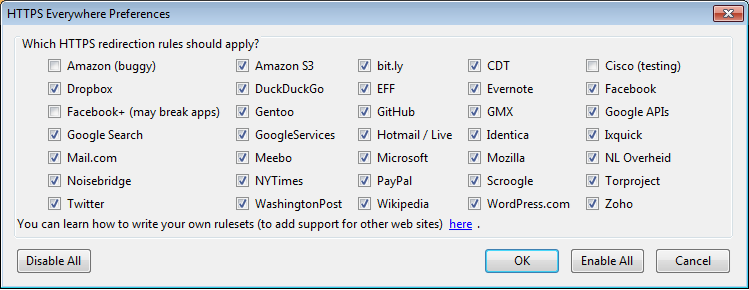
\includegraphics{https_everywhere_4.png}
\caption{HTTPS Everywhere}
\end{figure}

A list of all supported Web sites where HTTPS redirection rules should
be applied will be displayed. If you have problems with a specific
redirection rule, you can uncheck it here. In that case, HTTPS
Everywhere will no longer modify your connections to that specific site.

\subsection{Usage}

Once enabled and configured, HTTPS Everywhere is very easy and
transparent to use. Type an insecure HTTP URL (for example,
\href{http://www.google.com}{http://www.google.com}).

\begin{figure}[htbp]
\centering
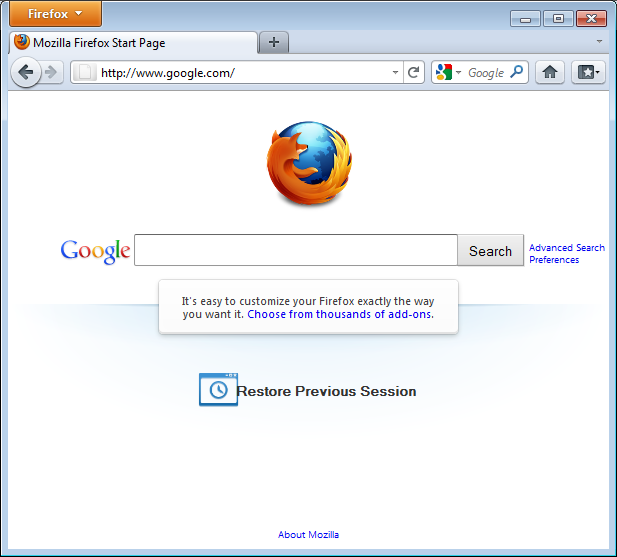
\includegraphics{https_everywhere_5.png}
\caption{HTTPS Everywhere}
\end{figure}

Press Enter. You will be automatically redirected to the secure HTTPS
encrypted Web site (in this example:
\href{https://encrypted.google.com}{https://encrypted.google.com}). No
other action is needed.

\begin{figure}[htbp]
\centering
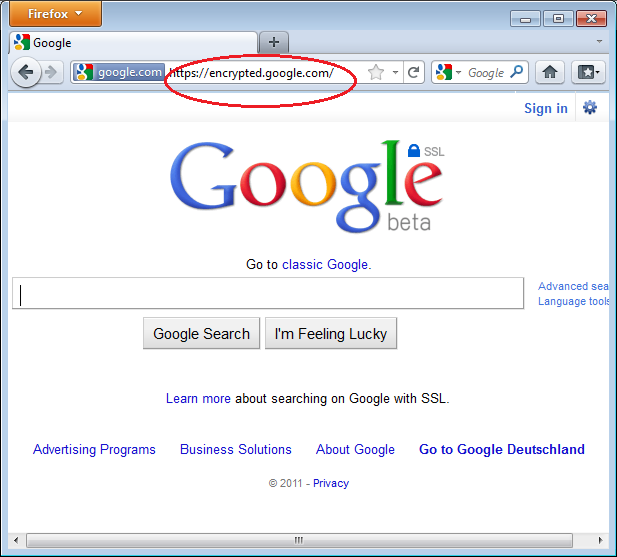
\includegraphics{https_everywhere_6.png}
\caption{HTTPS Everywhere}
\end{figure}

\subsection{If networks block HTTPS}

Your network operator may decide to block the secure versions of Web
sites in order to increase its ability to spy on what you do. In such
cases, HTTPS Everywhere could prevent you from using these sites because
it forces your browser to use only the secure version of these sites,
never the insecure version. (For example, we heard about an airport WiFi
network where all HTTP connections were permitted, but not HTTPS
connections. Perhaps the WiFi operators were interested in watching what
users did. At that airport, users with HTTPS Everywhere were not able to
use certain Web sites unless they temporarily disabled HTTPS
Everywhere.)

In this scenario, you might choose to use HTTPS Everywhere together with
a circumvention technology such as Tor or a VPN in order to bypass the
network's blocking of secure access to Web sites.

\subsection{Adding support for additional sites in HTTPS Everywhere}

You can add your own rules to the HTTPS Everywhere add-on for your
favorite Web sites. You can find out how to do that at:
\href{https://www.eff.org/https-everywhere/rulesets}{https://www.eff.org/https-everywhere/rulesets}.
The benefit of adding rules is that they teach HTTPS Everywhere how to
ensure that your access to these sites is secure. But remember: HTTPS
Everywhere does not allow you to access sites securely unless the site
operators have already chosen to make their sites available through
HTTPS. If a site does not support HTTPS, there is no benefit to adding a
ruleset for it.

If you are managing a Web site and have made an HTTPS version of the
site available, a good practice would be to submit your Web site to the
official HTTPS Everywhere release.

\subsection{Adblock Plus}

Adblock Plus
(\href{http://www.adblockplus.org}{http://www.adblockplus.org}) is
mainly known for blocking advertisements on websites. But it also can be
used to block other content that may try to track you. To keep current
with the latest threats, Adblock Plus relies on blacklists maintained by
volunteers.

Extra Geek info: How does Adblock Plus block addresses?

The hard work here is actually done by Gecko, the engine on top of which
Firefox, Thunderbird and other applications are built. It allows
something called ``content policies''. A content policy is simply a
JavaScript (or C++) object that gets called whenever the browser needs
to load something. It can then look at the address that should be loaded
and some other data and decide whether it should be allowed. There is a
number of built-in content policies (when you define which sites
shouldn't be allowed to load images in Firefox or SeaMonkey, you are
actually configuring one of these built-in content policies) and any
extension can register one. So all that Adblock Plus has to do is to
register its content policy, other than that there is only application
logic to decide which addresses to block and user interface code to
allow configuration of filters.

\subsection{Getting started with Adblock Plus}

Once you have Firefox installed:

\begin{enumerate}[1.]
\item
  Download the latest version of Adblock Plus from the Add-On database
  of Firefox
\item
  Confirm that your want Adblock Plus by clicking ``Install Now''.
\item
  After Adblock Plus has been installed, Firefox will ask to restart.
\end{enumerate}
\subsection{Choosing a filter subscription}

Adblock Plus by itself doesn't do anything. It can see each element that
a Web site attempts to load, but it doesn't know which ones should be
blocked. This is what Adblock's filters are for. After restarting
Firefox, you will be asked to choose a filter subscription (free).

\begin{figure}[htbp]
\centering
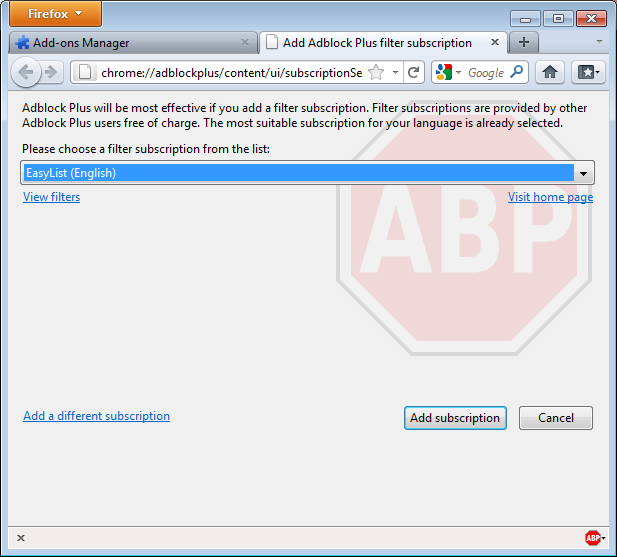
\includegraphics{abp_1.png}
\caption{Ad Block Plus}
\end{figure}

Which filter subscription should you choose? Adblock Plus offers a few
in its dropdown menu and you may wish to learn about the strengths of
each. A good filter to start protecting your privacy is EasyList (also
available at
\href{http://easylist.adblockplus.org/en}{http://easylist.adblockplus.org/en}).

As tempting as it may seem, don't add as many subscriptions as you can
get, since some may overlap, resulting in unexpected outcomes. EasyList
(mainly targeted at English-language sites) works well with other
EasyList extensions (such as region-specific lists like RuAdList or
thematic lists like EasyPrivacy). But it collides with Fanboy's List
(another list with main focus on English-language sites).

You can always change your filter subscriptions at any time within
preferences. Once you've made your changes, click OK.

\subsection{Creating personalized filters}

AdBlock Plus also lets you create your own filters, if you are so
inclined. To add a filter, start with Adblock Plus preferences and click
on ``Add Filter'' at the bottom left corner of the window. Personalized
filters may not replace the benefits of well-maintained blacklists like
EasyList, but they're very useful for blocking specific content that
isn't covered in the public lists. For example, if you wanted to prevent
interaction with Facebook from other Web sites, you could add the
following filter:

\begin{verbatim}
||facebook.*$domain=~facebook.com|~127.0.0.1
\end{verbatim}
The first part (\verb!||facebook.*!) will initially block everything
coming from Facebook's domain. The second part
(\verb!$domain=~facebook.com|~127.0.0.1!) is an exception that tells the
filter to allow Facebook requests only when you are in Facebook or if
the Facebook requests come from 127.0.0.1 (your own computer) in order
to keep certain features of Facebook working.

A guide on how to create your own Adblock Plus filters can be found at
\href{http://adblockplus.org/en/filters}{http://adblockplus.org/en/filters}.

\subsection{Enabling and disabling AdBlock Plus for specific elements or
Web sites}

You can see the elements identified by AdBlock Plus by clicking on the
ABP icon AdBlock Plus icon in your browser (usually next to the search
bar) and selecting ``Open blockable items''. A window at the bottom of
your browser will let you enable or disable each element on a
case-by-case basis. Alternatively, you can disable AdBlock Plus for a
specific domain or page by clicking on the ABP icon and ticking the
option ``Disable on {[}domain name{]}'' or ``Disable on this page
only''.

\subsection{Other extensions that can improve your security}

Below is a short list of extensions that are not covered in this book
but are helpful to further protect you.

\begin{itemize}
\item
  \textbf{Flagfox} - puts a flag in the location bar telling you where
  the server you are visiting is most probably located.
  \href{https://addons.mozilla.org/en-US/firefox/addon/flagfox/}{https://addons.mozilla.org/en-US/firefox/addon/flagfox/}
\item
  \textbf{BetterPrivacy} - manages ``cookies'' used to track you while
  visiting websites. Cookies are small bits of information stored in
  your browser. Some of them are used to track the sites you are
  visiting by advertisers.
  \href{https://addons.mozilla.org/en-US/firefox/addon/betterprivacy/}{https://addons.mozilla.org/en-US/firefox/addon/betterprivacy/}
\item
  \textbf{GoogleSharing} - If you are worried that google knows your
  search history, this extension will help you prevent that.
  \href{https://addons.mozilla.org/en-us/firefox/addon/googlesharing/}{https://addons.mozilla.org/en-us/firefox/addon/googlesharing/}
\end{itemize}
